%\documentclass[a4paper,oneside,onecolumn]{article}
\documentclass[journal=nalefd,manuscript=letter]{achemso}
\usepackage{graphicx}
\usepackage{amsmath}
\usepackage{amssymb}
\usepackage{subfigure}
%\usepackage{epstopdf}
%\usepackage{setspace}
%\onehalfspace
%\usepackage{authblk}
%\usepackage[margin=2.3cm]{geometry}

%\geometry{a4paper,left=2.3cm,right=2.3cm,top=2.5cm,bottom=4.5cm}

\usepackage[version=3]{mhchem} % Formula subscripts using \ce{}
\usepackage[T1]{fontenc}       % Use modern font encodings
\renewcommand{\figurename}{Figure S}
\newcommand{\nm}{\ensuremath{\,\textrm{nm}}}
\newcommand{\eV}{\ensuremath{\,\textrm{eV}}}
\newcommand{\uM}{\ensuremath{\,\mu\textrm{M}}}
\newcommand{\uW}{\ensuremath{\,\mu\textrm{W}}}
\newcommand{\meV}{\ensuremath{\,\textrm{meV}}}

\author{Aquiles Carattino}
\affiliation[Leiden]
{Huygens-Kamerlingh Onnes, Leiden, The Netherlands}
\author{Saumyakanti Khatua}
\affiliation{Indian Institute of Technology- Gandhinagar, Ahmedabad,  India}
\author{Michel Orrit}
\email{orrit@physics.leidenuniv.nl}
\affiliation[Leiden]
{Huygens-Kamerlingh Onnes, Leiden, The Netherlands}

\title{Supplementary information for: \textit{In situ} tuning of gold nanorod plasmon through oxidative cyanide
etching}

\begin{document}
\maketitle

\section{Solution Results}
\begin{figure}[htp]
 \centering
 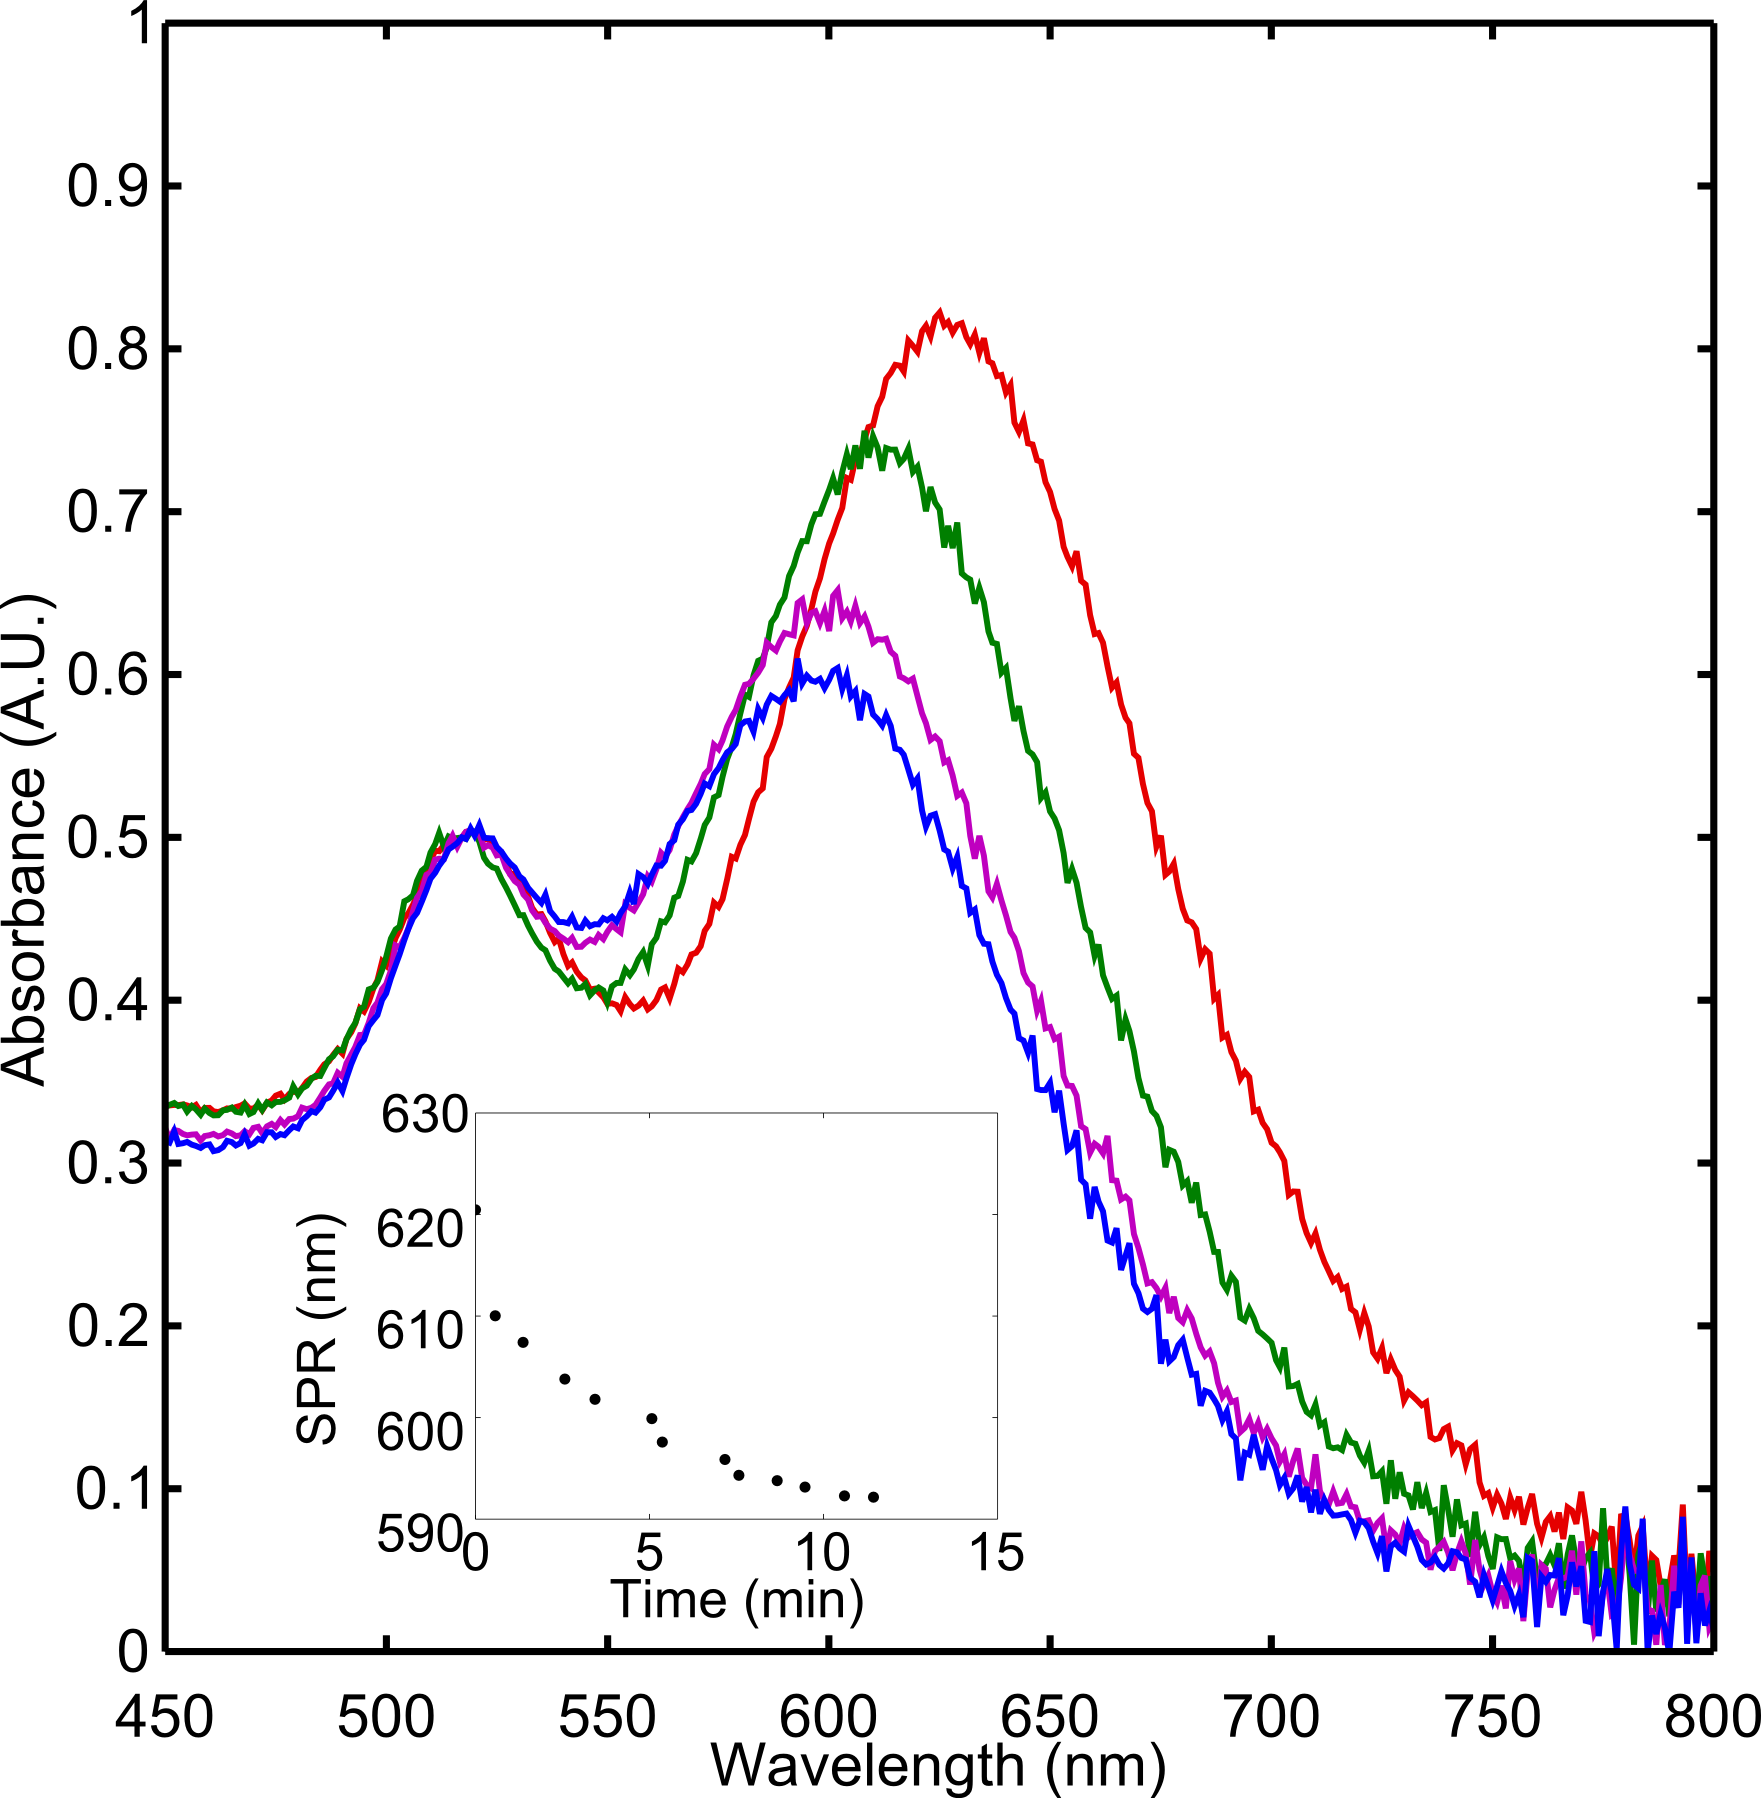
\includegraphics[width=0.45\linewidth]{Figures/04_Supporting/01_Bulk/01_bulk.png}
 \caption{Extinction spectra of a bulk suspension of gold nanorods dispersed in
 $100\uM$ KCN. The curves are displayed at 2 minutes intervals. The
 inset shows the peak position as a function of time. The curves were normalized
 to the transverse peak for clarity.}
 \label{fig:Bulk}
\end{figure}

Figure S\ref{fig:Bulk} shows the behavior of the same nanorods dispersed in
$100\uM$ KCN. We observe a clear blue shift of the longitudinal plasmon
resonance, towards the transverse peak at around $530\nm$. As stated in the main
text, we attribute the blue shift of the peak to a shortening of the long axis
of the rods. This is because the CTAB is more efficient in protecting the sides
than the tips of the particles. The blue shift does not seem stabilized for the last spectrum. We attribute this to a complete consumption of KCN by excess gold metal in our sample. If more KCN had been added, the blue-shift would probably have continued.

The spectra were acquired in an UV-Vis spectrometer. The first spectrum was
acquired with the rods dispersed in water, before adding KCN into the cuvette.
Later a solution such that the final concentration was $100\uM$ was added and a
set of automatic spectra was recorded at a fixed interval of time. The peak
position was extracted by fitting a double Lorentzian, one with a fixed central
wavelength (the transverse resonance) and a second one for the longitudinal
plasmon.


\section{SEM Images}

\begin{figure}[htp]
 \centering
 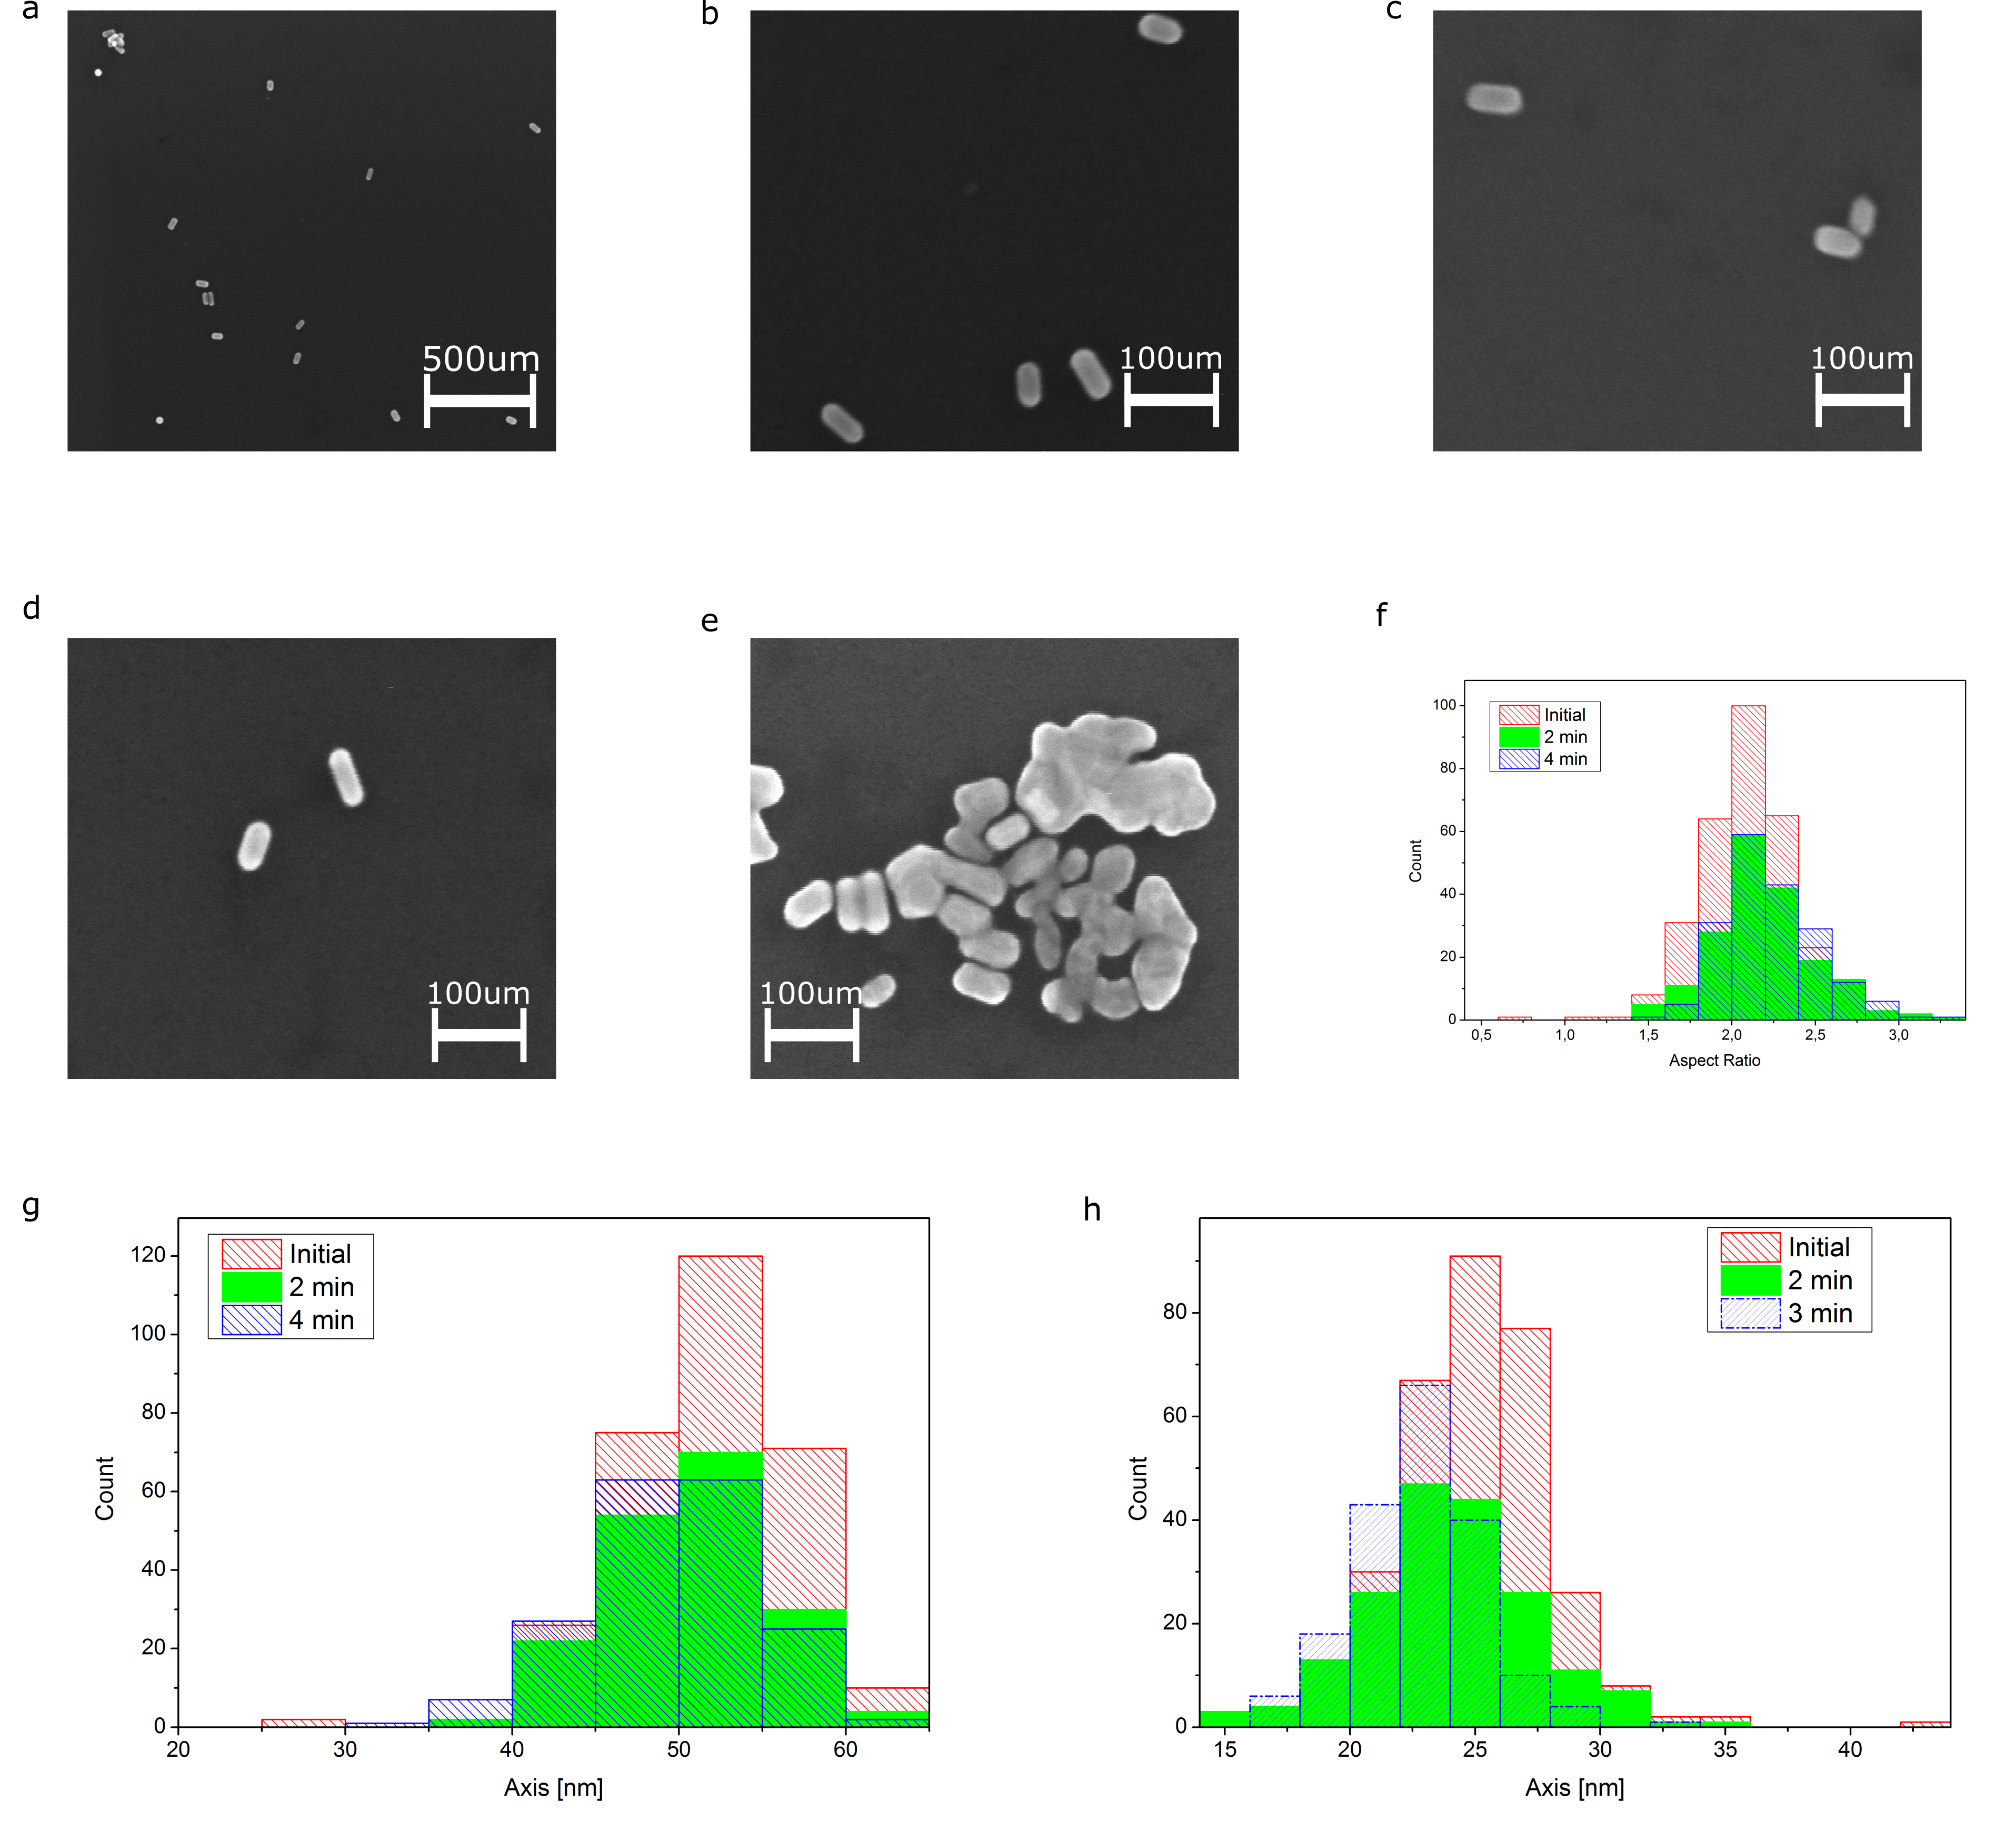
\includegraphics[width=0.95\linewidth]{Figures/04_Supporting/02_SEM/sem.png}
 \caption{SEM images of the rods a) after synthesis, b) after $2$ minutes in
 $20\uM$ KCN when particles are separated, c) or when they form clusters. d)
 separated particles after $4$ minutes in KCN and e) when they were forming
 clusters. f-h) Histograms of the aspect ratio (f), longitudinal(g) and
 transverse axis(h) before, after $2$ and after $4$ minutes in KCN. The
 distribution of values is too broad to visualize a shift in aspect ratio.
 Statistics on the values, however, show a slight increase and the data is
 summarized in table 1. }
 \label{fig:SEM}
\end{figure}

Figure S\ref{fig:SEM} shows the SEM images of the rods. In S\ref{fig:SEM}a an
example of the rods after synthesis and before etching. Figures S\ref{fig:SEM}b
and S\ref{fig:SEM}c are after $2$ minutes in $20\uM$ KCN and the difference on
the shape of the particles when they are separated from each other and in
contact is notable. Figures S\ref{fig:SEM}d and S\ref{fig:SEM}e were taken after
$4$ minutes in KCN. The histograms in Figures S\ref{fig:SEM}f-h show the
analysis of the aspect ratio, the longitudinal and the transverse axes
respectively for each of the cases. Table 1 summarizes the average values found
after analyzing approximately $300$ particles. The shift is rather small as
compared to the standard deviation of the distribution of sizes.

\begin{table}[htp]
\begin{tabular*}{0.48\textwidth}{c c c c c}
 $\,$ & L (nm) & Sdv (nm) & D (nm) & Sdv (nm) \\\hline
 $0\textrm{min}$ & $51$ & $5$ & $24$ & $3$ \\
 $2\textrm{min}$ & $50$ & $5$ & $23$ & $3$ \\
 $4\textrm{min}$ & $49$ & $5$ & $22$ & $2$ \\
\end{tabular*}
\label{tab:SEM_results}
\caption{Summary of the results obtained for 300 different particles while
imaging them with an SEM. L and D are the length and diameter respectively.
Sdv is the standard deviation of the values}
\end{table}

\section{Background Spectrum}
\begin{figure}[htp]
 \centering
 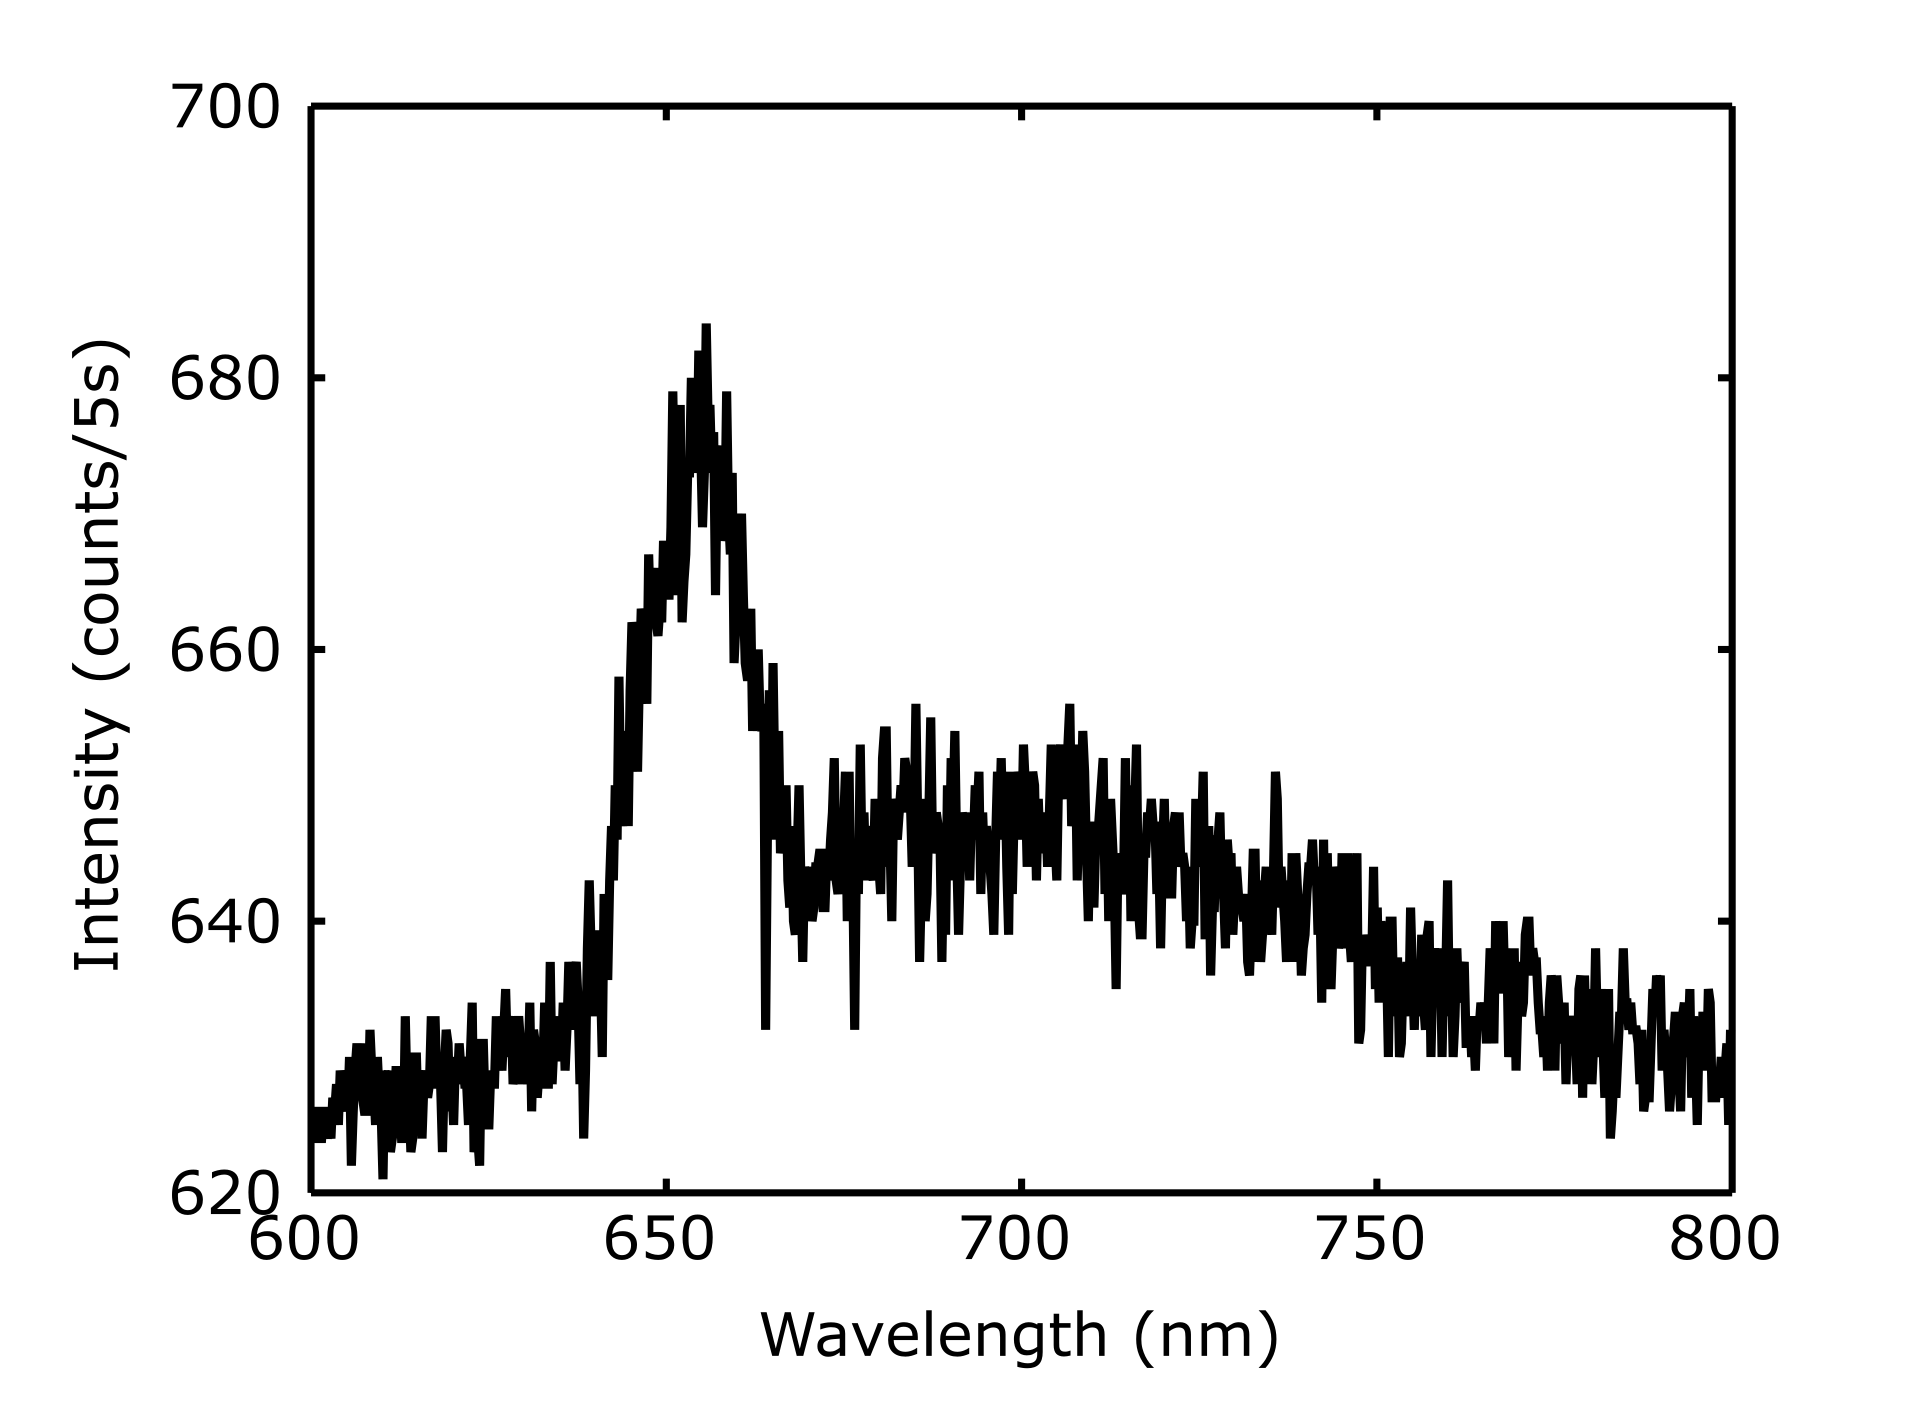
\includegraphics[width=0.95\linewidth]{Figures/04_Supporting/03_Background/background.png}
 \caption{Spectra from the background while exciting with a $532\nm$ laser. The
 peak appearing at $650\nm$ is attributed to Raman scattering from the O-H stretching modes of water.}
 \label{fig:Background}
\end{figure}

Figure S\ref{fig:Background} shows the typical background when exciting with a
$532\nm$ laser. The peak at $650\nm$ is attributed to Raman scattering from
water. Normally this background can be well subtracted from the spectra acquired
on particles. For less intense curves however, it is possible to observe
shoulder appearing at this particular wavelength. This indicates a non-additive 
phenomenon that we attributed to enhanced Raman scattering close to the nanoparticles.

\end{document}
